\section*{Problem 2}

Give a chip design containing three power components and eight regular components satisfying the following constraints:
\begin{itemize}
  \item The width of the chip is 29 and the height is 22.
  \item All power components have width 4 and height 2.
  \item The sizes of the eight regular components are $9 \times 7$, $12 \times 6$, $10 \times 7$, $18 \times 5$, $20 \times 4$, $10 \times 6$, $8 \times 6$ and $10 \times 8$, respectively.
  \item All components may be turned 90, but may not overlap.
  \item In order to get power, all regular components should directly be connected to a power component, that is, an edge of the component should have at least one point in common with an edge of the power component.
  \item Due to limits on heat production the power components should be not too close: their centres should differ at least 17 in either the $x$ direction or the $y$ direction (or both).
\end{itemize}

\vspace{4mm}

\subsection*{Solution:}
First of all, we generalize this problem for any width $S_1$ and height $S_2$ of the chip and for any number $p$ and $r$ of power and regular components respectively. Assume the chip plan is a positive plane whose left-bottom corner has coordinate $(0, 0)$, then the right-top corner has coordinate $(S_1, S_2)$.
Next, we introduce $2 \times p$ coordinates of the form $(x_{ik}, y_{ik})$ for $i = 1, 2 , ... , p$ and $k = 1, 2$, to represent the corners of each power component. Hence, power component $i$ has coordinates $(x_{i1}, y_{i1})$, $(x_{i2}, y_{i1})$, $(x_{i1}, y_{i2})$ and $(x_{i2}, y_{i2})$.

Similarly, we introduce $2 \times r$ coordinates of the form $(n_{jk}, m_{jk})$ for $j = 1, 2 , ... , r$ and $k = 1, 2$, to represent the corners of each regular component.

Now, we give formulas that translates the constraints in terms of this variables.

\begin{description}
  \item[Constraint 1:] The chip is a positive plane, so all the coordinates should be positive. Additionally, the width of the chip is $S_1$ and the height is $S_2$.

  Then we have
  \[  \bigwedge_{i=1}^p S_1 \geq x_{i2} \geq x_{i1} \geq 0 \wedge S_2 \geq y_{i2} \geq y_{i1} \geq 0 \;\; \wedge \]
  \[  \bigwedge_{i=1}^r S_1 \geq n_{i2} \geq n_{i1} \geq 0 \wedge S_2 \geq m_{i2} \geq m_{i1} \geq 0 \]


  \item[Constraint 2:] All coordinates of a given component have to respect its respective size, also a component may be turned 90. To formulate this, we define $Z_1$ and $Z_2$ as the height and width of all power components, and $H_{j}$ and $W_{j}$ as the height and width of regular component $j$.

  Then we have the following formula for power components:
  \[  \bigwedge_{i=1}^p ((x_{i2} - x_{i1} = Z_1 \; \wedge \; y_{i2} - y_{i1} = Z_2) \;\; \vee \]
  \[ (x_{i2} - x_{i1} = Z_2 \; \wedge \; y_{i2} - y_{i1} = Z_1)) \]

  Similarly, the formula for regular components is:
  \[  \bigwedge_{j=1}^r (n_{j2} - n_{j1} = W_j \; \wedge \; m_{j2} - m_{j1} = H_j) \;\; \vee (n_{j2} - n_{j1} = H_j \; \wedge \; m_{j2} - m_{j1} = W_j) \]


  \item[Constraint 3:] All components may not overlap.

\begin{center}
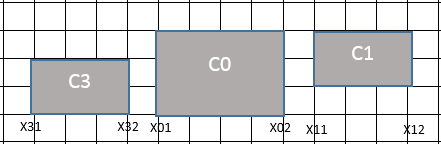
\includegraphics[width=0.5\textwidth]{Part1_2_1.png}
\end{center}
  As the figure shows, only if a component's $x_{i1}$ is larger than the other one's $x_{k2}$, then these two components are not overlapped. We also have the case in the $y$ direction. Hence the formulas that express the two components may not overlap are the following.

  Among the power components:

  \[  \bigwedge_{i,l: 1 \leq i < l \leq p}
  x_{i2} \leq x_{l1} \; \vee \; x_{l2} \leq x_{i1} \; \vee \; y_{i2} \leq y_{l1} \; \vee \; y_{l2} \leq y_{i1} \]

  Among the regular components:

  \[  \bigwedge_{j,l: 1 \leq j < l \leq r}
  n_{j2} \leq n_{l1} \; \vee \; n_{l2} \leq n_{j1} \; \vee \; m_{j2} \leq m_{l1} \; \vee \; m_{l2} \leq m_{j1}  \]

  Between the power components and the regular components:

  \[  \bigwedge_{i,k: 1 \leq i \leq p, 1 \leq j \leq r}
   x_{i2} \leq n_{j1} \; \vee \; n_{j2} \leq x_{i1} \; \vee \; y_{i2} \leq m_{j1} \; \vee \; m_{j2} \leq y_{i1} \]

  \item[Constraint 4:] An edge of the regular component should have at least one point in common with an edge of the power component.

\begin{center}
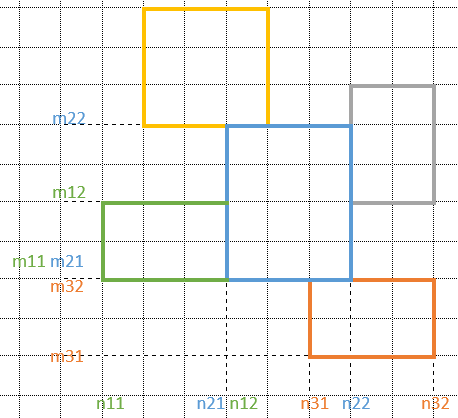
\includegraphics[width=0.5\textwidth]{Part1_2_2.png}
\end{center}

  As the figure shows, if two components are touched at least by one point, then at least one coordinate of a component is the same as the other one. Based on this observation, we can state that when the $x$ coordinates of two components are the same, and also the $y$'s coordinate of one is bound by the $y$'s coordinates of the other component, we can conclude that they are touching. The same holds when they share a $y$'s coordinate. We denote this condition as follows.

  \[  \bigwedge_{i,k: 1 \leq i \leq p, 1 \leq k \leq r}
  ((x_{i2} = n_{k1} \; \vee \; x_{i1} = n_{k2}) \; \wedge \;
  (y_{i2} \geq m_{k1} \wedge m_{k2} \geq y_{i1}) \; \vee \; \]
  \[  ((y_{i2} = m_{k1} \; \vee \; y_{i1} = m_{k2}) \; \wedge \;
  (x_{i2} \geq n_{k1} \wedge n_{k2} \geq x_{i1}))) \]

  \item[Constraint 5:] The power components' centres should differ at least 17 in either the $x$ direction or the $y$ direction (or both).

  The centers of the power components are $(x_{i1} + \frac{x_{i2} - x_{i1}}{2}, y_{i1} + \frac{y_{i2} - y_{i1}}{2} )$.

  For each pair of the power components, we have

  \[  \bigwedge_{i,k: 1 \leq i < k \leq p}
  [ (x_{i1} + \frac{x_{i2} - x_{i1}}{2}) - (x_{k1} + \frac{x_{k2} - x_{k1}}{2}) \geq 17 \; \vee \; \]
  \[ (x_{k1} + \frac{x_{k2} - x_{k1}}{2}) - (x_{i1} + \frac{x_{i2} - x_{i1}}{2}) \geq 17 \; \vee \; \]
  \[ (y_{k1} + \frac{y_{k2} - y_{k1}}{2}) - (y_{i1} + \frac{y_{i2} - y_{i1}}{2}) \geq 17 \; \vee \; \]
  \[ (y_{i1} + \frac{y_{i2} - y_{i1}}{2}) - (y_{k1} + \frac{y_{k2} - y_{k1}}{2}) \geq 17 ] \]


\end{description}

The total formula now consists of the conjunction of all these clauses. To solve this particular problem, we made the Yices smt code considering the number of power components $p=3$, the number of regular components $r=8$, and replacing the parameters $S_1$, $S_2$, $Z_1$, $Z_2$, $H_j$ and $W_j$ with its own values of height and width as specified by the problem.

This is expressed in SMT syntax as follow:

{\footnotesize

{\tt (benchmark Part1\_2.smt}

{\tt :logic $QF\_LIA$}

{\tt :extrafuns (}

{\tt (x11 Int) (x12 Int) (y11 Int) (y12 Int)}

{\tt (x21 Int) (x22 Int) (y21 Int) (y22 Int)}

$\cdots \cdots$

{\tt (n81 Int) (n82 Int) (m81 Int) (m82 Int)}

{\tt )}

{\tt :formula (and}

{\tt (>= 29 x12) (>= x12 x11) (>= x11 0) (>= 22 y12) (>= y12 y11) (>= y11 0)}

{\tt (>= 29 x22) (>= x22 x21) (>= x21 0) (>= 22 y22) (>= y22 y21) (>= y21 0)}

$\cdots \cdots$

{\tt (>= 29 n82) (>= n82 n81) (>= n81 0) (>= 22 m82) (>= m82 m81) (>= m81 0)}

{\tt (or (and (>= 29 x12) (>= 22 y12) (= (- x12 x11) 4) (= (- y12 y11) 2))}

{\tt (and (>= 22 x12) (>= 29 y12) (= (- y12 y11) 4) (= (- x12 x11) 2)))}

$\cdots \cdots$

{\tt (or (and (= (- x32 x31) 4) (= (- y32 y31) 2)) (and (= (- x32 x31) 2) (= (- y32 y31) 4)))}

{\tt (or (and (= (- n12 n11) 9) (= (- m12 m11) 7)) (and (= (- n12 n11) 7) (= (- m12 m11) 9)))}

$\cdots \cdots$

{\tt (or (and (= (- n82 n81) 10) (= (- m82 m81) 8)) (and (= (- n82 n81) 8) (= (- m82 m81) 10)))}

{\tt ;; not overlap among power components}

{\tt (or (<= x12 x21) (<= x22 x11) (<= y12 y21) (<= y22 y11))}

{\tt (or (<= x12 x31) (<= x32 x11) (<= y12 y31) (<= y32 y11))}

{\tt (or (<= x32 x21) (<= x22 x31) (<= y32 y21) (<= y22 y31))}

{\tt ;; not overlap among regular components}

{\tt (or (<= n12 n21) (<= n22 n11) (<= m12 m21) (<= m22 m11))}

{\tt (or (<= n12 n31) (<= n32 n11) (<= m12 m31) (<= m32 m11))}

$\cdots \cdots$

{\tt (or (<= n72 n81) (<= n82 n71) (<= m72 m81) (<= m82 m71))}

{\tt ;;not overlap between power components and regular ones}

{\tt (or (<= x12 n11) (<= n12 x11) (<= y12 m11) (<= m12 y11))}

{\tt (or (<= x12 n21) (<= n22 x11) (<= y12 m21) (<= m22 y11))}

$\cdots \cdots$

{\tt (or (<= x32 n81) (<= n82 x31) (<= y32 m81) (<= m82 y31))}

{\tt ;;Constraint 4}

{\tt (or}

{\tt (and (or (= x11 n12) (= x12 n11)) (not (or (< y12 m11) (> y11 m12))))}

{\tt (and (or (= x21 n12) (= x22 n11)) (not (or (< y22 m11) (> y21 m12))))}

$\cdots \cdots$

{\tt (and (or (= y31 m12) (= y32 m11)) (not (or (< x32 n11) (> x31 n12))))}

{\tt )}

$\cdots \cdots$

{\tt (or}

{\tt (and (or (= x11 n82) (= x12 n81)) (not (or (< y12 m81) (> y11 m82))))}

{\tt (and (or (= x21 n82) (= x22 n81)) (not (or (< y22 m81) (> y21 m82))))}

$\cdots \cdots$

{\tt (and (or (= y31 m82) (= y32 m81)) (not (or (< x32 n81) (> x31 n82))))}

{\tt )}

{\tt ;;Constraint 5}

{\tt (or (>= (- (+ x11 (/ (- x12 x11) 2)) (+ x21 (/ (- x22 x21) 2))) 17)}

{\tt (>= (- (+ x21 (/ (- x22 x21) 2)) (+ x11 (/ (- x12 x11) 2))) 17)}

{\tt (>= (- (+ y11 (/ (- y12 y11) 2)) (+ y21 (/ (- y22 y21) 2))) 17)}

{\tt (>= (- (+ y21 (/ (- y22 y21) 2)) (+ y11 (/ (- y12 y11) 2))) 17))}

$\cdots \cdots$

{\tt (or (>= (- (+ x11 (/ (- x12 x11) 2)) (+ x31 (/ (- x32 x31) 2))) 17)}

{\tt (>= (- (+ x31 (/ (- x32 x31) 2)) (+ x11 (/ (- x12 x11) 2))) 17)}

{\tt (>= (- (+ y11 (/ (- y12 y11) 2)) (+ y31 (/ (- y32 y31) 2))) 17)}

{\tt (>= (- (+ y31 (/ (- y32 y31) 2)) (+ y11 (/ (- y12 y11) 2))) 17))}

{\tt ))}
}

Applying {\tt yices-smt -m part$1\_2$.smt}, we test out a satisfiable chip design plan.

{\footnotesize

{\tt sat}

{\tt(= x11 4)}

{\tt(= x12 6)}

{\tt(= y11 2)}

{\tt(= y12 6)}

{\tt(= x21 0)}

{\tt(= x22 4)}

{\tt(= y21 20)}

{\tt(= y22 22)}

{\tt(= x31 21)}

{\tt(= x32 23)}

$\cdots \cdots$

}

The following picture illustrates the solution of this problem given by the tool.

\begin{center}
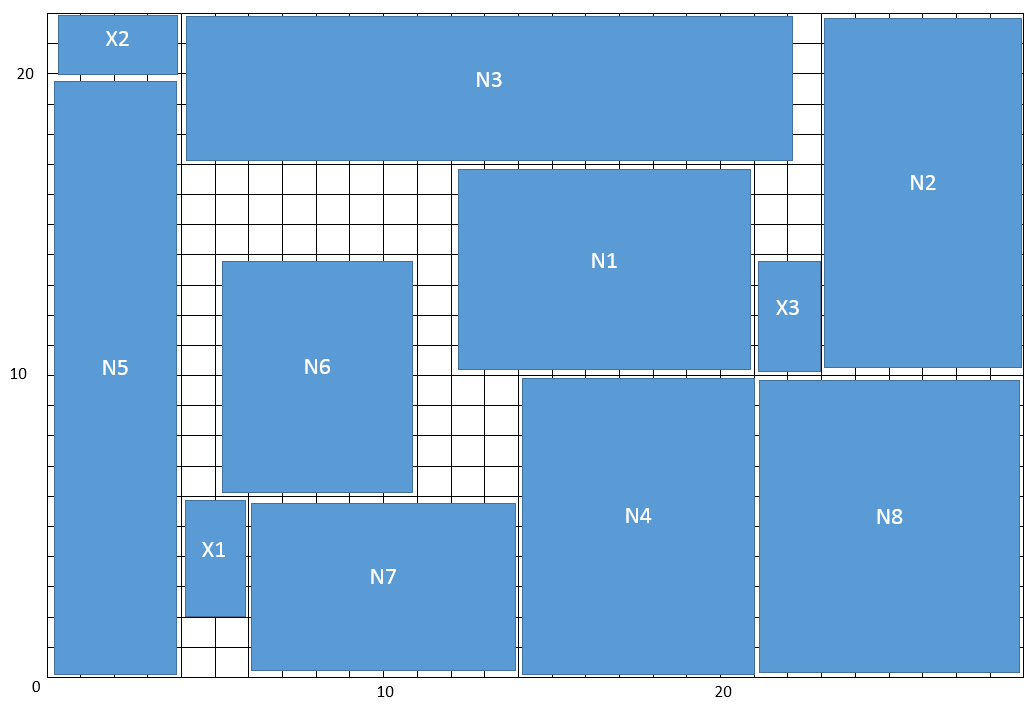
\includegraphics[width=0.8\textwidth]{Part1_2_3.png}
\end{center}

\subsection*{Remark:}


\subsection*{Generalization:} 
We generalized our approach for any composition of a chip, some power components and regular components with known sizes to test if it is possible to obtain a fine chip design. Regardless the size of the chip and these components and the number of the components, this approach specifies two more constraints. One is the safe distance for the power components due to heat production. The other is the common touching between power components and regular components. These two constraints are derived from the characteristics of the components to apply to the chip. Different components have different characteristics, which may require different clauses to formulate. This is the limitation of our generalization. The satisfiability for a good chip design highly depends on the size of the components.




